\label{sec:rq3}

\begin{figure}[htbp]
\centering
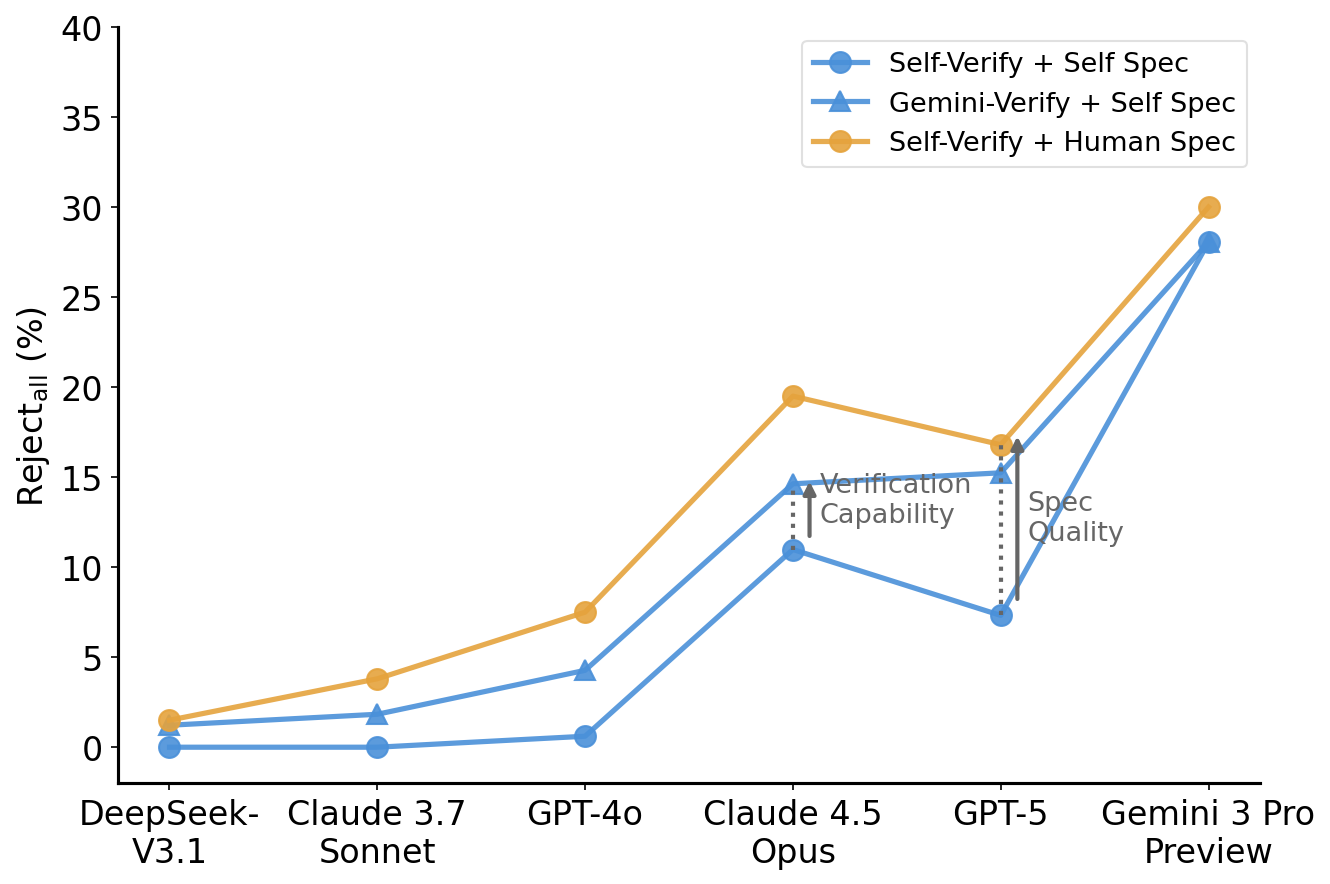
\includegraphics[width=1.0\linewidth]{images/ablation_study.png}
\caption{Ablation study disentangling specification quality and verification capability.
Compared to the \emph{Self-Verify + Self Spec} baseline, using human-written specifications improves performance by $+5.08$ percentage points, while replacing self-verification with a stronger verifier improves performance by $+3.05$ percentage points.
Both factors significantly impact performance.}
\label{fig:ablation}
\end{figure}

\begin{tcolorbox}[
  colback=gray!10,
  colframe=gray!60,
  boxrule=0.6pt,
  arc=2pt,
  left=6pt,
  right=6pt,
  top=6pt,
  bottom=6pt
]
\small
\textbf{Verification Complexity Trade-off.} The harder the verification task, the stronger the prover required, and the more difficult it becomes to accurately assess specification quality. Even when the verification objective perfectly captures specification correctness, overly complex proof obligations risk systematic underestimation, rendering such benchmarks unreliable metrics for specification generation.
\label{trade-off}
\end{tcolorbox}



Compared to \textsc{Clever}'s end-to-end approach, which achieves only 0.621\% correctness and provides virtually no discriminative power across models, \textsc{Coins} successfully differentiates specification generation capabilities among all six models. As shown in Table~\ref{tab:generation}, \textsc{Reject}$_{\text{all}}$ rates range from 1.22\% (DeepSeek-V3.1) to 28.05\% (Gemini 3 Pro Preview), demonstrating meaningful variance across the model spectrum.

However, even the task of verifying test case acceptance proves highly challenging. Table~\ref{tab:verification} and Table~\ref{tab:generation} reveal that while models can often verify individual test cases, consistent verification across all cases remains elusive. This makes it difficult to determine whether failures stem from proof synthesis limitations or genuine specification defects.

To disentangle these factors, we conduct an ablation study with two controlled interventions (Figure~\ref{fig:ablation}).
We start from a baseline where each model verifies its own generated specifications (\emph{Self-Verify + Self Spec}).
We then separately improve either verification capability by replacing self-verification with Gemini~3~Pro~Preview (\emph{Gemini-Verify + Self Spec}), or specification quality by substituting LLM-generated specifications with human-written references (\emph{Self-Verify + Human Spec}).

Both factors significantly affect performance.
Improving specification quality yields an average gain of $+5.08$ percentage points, while stronger verification contributes $+3.05$ percentage points.
Although the former has a larger impact, verification capability remains a substantial factor even for test case acceptance.
